\documentclass[letterpaper]{article}
\usepackage[T1]{fontenc}
\usepackage[pdfusetitle,colorlinks]{hyperref}
\usepackage[pdftex]{graphicx}
\usepackage{verbatim}
\usepackage{amsmath}
\usepackage{booktabs}
\usepackage[font=scriptsize,labelfont=bf,margin=3em]{caption}

\newcommand{\cpp}{C{\nobreak+}{\nobreak+}}

\newcommand{\code}[1]{\small\textsf{#1}}

\renewcommand{\_}{\allowbreak\textunderscore\allowbreak}


\title{Genetic Chess}
\author{Mark Harrison}
\date{}

\begin{document}

\maketitle

\begin{abstract}
This work is a program for evolving chess-playing AIs.  By pitting a population of AIs against each other in chess matches, killing off the losers, and breeding the winners, it is hoped that one specimen will be able to stand up against a more traditionally developed engine (if only on the easiest difficulty setting). Though it is written in \cpp{}, it is the hope of the author that the style and architecture are comprehensible.
\end{abstract}

\tableofcontents{}


\section{Building}

\subsection{Linux}
Required software: GCC\footnote{\url{https://gcc.gnu.org/}} or clang\footnote{\url{https://clang.llvm.org/}}, latexmk\footnote{\url{https://ctan.org/pkg/latexmk}}, and doxygen\footnote{\label{doxygen-footnote}\url{http://www.doxygen.nl/}} (the last two are for generating the documentation). All of these should be available in your OS's package manager.

\begin{enumerate}
	\item After cloning the project, run \code{python create\_Makefile.py [compiler]} to regenerate the Makefile. The choices for the compiler are \code{gcc} and \code{clang}.
	\item Run \code{make}. Optional target arguments include
		\begin{itemize}
			\item \code{all}: The default, creates \code{release} and \code{debug} builds as well as the documentation: a PDF user manual and Doxygen code documentation in HTML.
			\item \code{release} The build that is optimized for speed.
			\item \code{debug} The build that contains symbols for debugging.
			\item \code{test}, \code{test\_release}, \code{test\_debug}: Runs test suites on the named builds to ensure proper functioning and to measure performance.
			\item \code{docs}, \code{user\_manual}, \code{code\_docs}: Generate documentation. The target \code{docs} implies the other two. The \code{user\_manual} is a PDF document detailing how to run the program; the \code{code\_docs} target is a series of HTML pages detailing the public interfaces of the \cpp{} code.
			\item \code{clean}, \code{clean\_release}, \code{clean\_debug}: Deletes build files and (in the case of \code{clean\_all}) generated documentation files.
		\end{itemize}
		\item The executable files will be placed in the directory \code{./bin/<compiler>/<build>/\allowbreak{}genetic\_chess}, where \code{<compiler>} is either \code{gcc} or \code{clang} from step 1 and \code{<build>} is either \code{release} or \code{debug}. For convenience, symbolic links to the last made executable file will placed in \code{./bin/<build>/}.
\end{enumerate}

\subsection{Windows}
Required software: Any \cpp{} development suite. The \code{.sln} and \code{.vcxproj} files are project files for Microsoft Visual Studio\footnote{\url{https://visualstudio.microsoft.com/}}. The user manual can be generated with TexMaker\footnote{\url{https://www.xm1math.net/texmaker/}} or any other \LaTeX{} suite. The code documentation is generated with Doxygen (see footnote \ref{doxygen-footnote}).


\section{Running}\label{running}

In the options below, words surrounded by angle brackets \code{<like this>} are meant to be replaced by a value for the option. If the word is also surrounded by straight brackets \code{[<like this>]}, then it can be omitted.

These first options are standalone operations. If multiple options are used, all besides the first are ignored.
\begin{description}
	\item[\code{genetic\_chess -help}] Print the help text that describes how to run the program.
	\item[\code{genetic\_chess -test}] Run tests of the program for chess rule conformance and for Genetic AIs working properly.
	\item[\code{genetic\_chess -perft}:] Test game logic and speed by counting legal moves from a list of board positions.
	\item[\code{genetic\_chess -speed}:] Measure the speed of various components of the chess engine.
	\item[\code{genetic\_chess -confirm <file name>}] Analyze a game record in Portable Game Notation (PGN \cite{pgn-file-format}) to check that all moves listed are legal and all move are correctly noted with respect to check (+), capture (x), and checkmate (\#).
	\item[\code{genetic\_chess -genepool <file name>}]
This will start up a gene pool with Genetic\_AIs playing against each other---mating, killing, mutating, all that good Darwinian stuff. The required file name parameter will cause the program to load a gene pool and other settings from a configuration file. A record of every genome and game played will be written to text files.
\end{description}
The following options can be used together to start a single chess game.
\begin{description}
	\item[\code{genetic\_chess <player> [<player>]}] Starts a local game. If two players are specified, the first parameter is the white player, and the second is black. If only one player is specified, the program waits for GUI input on stdin. The \code{<player>} argument is replaced with one of the following:
	\begin{description}
		\item[\code{-genetic [<file name> [<number>]]}:] a Genetic AI player. If a file name follows, load the genes from that file. If there are several genomes in a file, the file name can be followed by a number to load the genome with that ID\@. If no number is specified, then the last genome in the file is loaded (presumably this one is the most evolved).
		\item[\code{-random}:] an AI player that chooses a random legal move at each turn.
	\end{description}
\end{description}
Other game options that can be added:
\begin{description}
	\item[\code{-time <number>}:] The starting about of time on the game clocks in seconds.
	\item[\code{-repeat\_moves <number>}:] The number of moves a player must make before the clocks are reset to their starting time.
	\item[\code{-increment <number>}:] The amount of time to add to the clocks after every move.
	\item[\code{-board <FEN>}] A description of a board setup in \href{https://en.wikipedia.org/wiki/Forsyth\%E2\%80\%93Edwards_Notation}{Forsyth-Edwards Notation}~\cite{fen-notation} on which to start the game. The entire FEN should be quoted.
	\item[\code{-game\_file <file name>}] The name of a file for recording the moves of the game and other information. If the file exists, the game record will be appended.
\end{description}
Genetic Chess can communicate with GUI chess programs (xboard, PyChess, Cute Chess, and \href{https://lichess.org}{lichess.org} among others) through the \href{https://www.gnu.org/software/xboard/engine-intf.html}{Chess Engine Communication Protocol (CECP or, often, xboard)} or the \href{http://wbec-ridderkerk.nl/html/UCIProtocol.html}{Universal Chess Interface (UCI)}. When using Genetic Chess this way, only specify the arguments for a single player. The program will then wait for communication from the GUI through stdin.


\section{Non-Evolutionary Aspects}

These sections describe the aspects of the chess AI that are not genetically modifiable, usually because of at least one of the following reasons:
\begin{itemize}
	\item There is no sense in which the aspect of play is improvable. Any modification would be detrimental to the chess playing;
	\item It would take far too much time to evolve that aspect of play from a random starting configuration, or it would interfere too much with the evolution of other aspects;
	\item I cannot conceive of how to represent the state space of that particular play strategy so that it may be genetically encoded.
\end{itemize}
On the last point, it has been suggested to me that, instead of the specific genes listed in Section~\ref{gene-section}, the genes should encode more abstract and generic strategies and heuristics for evaluating a board state. While this would probably better mimic biological evolution (wherein adenine and thymine are rather neutral as to their teleology), I have no idea how to program such an abstract representation and how to translate the action of such genes into chess moves. So, what results from all this programming is a glorified tuning algorithm for parameters in predefined genes with hard-coded meanings.

On the other hand, so is every other genetic algorithm (see~\cite{evolved-antenna},~\cite{evolved-stellarator}, and others). Plus, these genes can evolve to have near-zero influence on game decisions, so these AIs are perfectly capable of telling me exactly what they think of my painstakingly crafted genes.\footnote{The little ingrates!}

\subsection{Endgame Scoring}

Winning gives a positive infinite score.
Losing gives a negative infinite score.
Draw gives zero.

Why not evolve these numbers? While the priorities of various genes can be varied to yield different playing styles, the only reasonable score to assign to a win is one that is larger than any other score. It can only be a disadvantage to prefer anything to a winning move. While this would result in upward evolutionary pressure on the score assigned to winning, it would stall the evolution of all other genes while the score assigned to winning was pushed high enough to always be preferred.

The specific values were chosen to make the scoring symmetrical between the two players, in that the score for one side is the negative of the score as seen from the other side (assuming the same player does the scoring). What is good for one player is bad for the other player by the same amount.

\subsection{Mini-maxing}\label{sec-minimax}

The principle behind the minimax algorithm is that the quality of a move is measured by the quality of moves it allows the opponent to make. Of course, the quality of those moves is measured by the quality of the moves that follow. Ideally, the only required board evaluation scores would be \(1\)~for a win, \(0\)~for a draw, and \(-1\)~for a loss, and all possible sequences of moves would be examined to find the guaranteed outcome. Unfortunately, the number of positions to examine in a typical game is far too large to examine in a few minutes, so the search has to be cut off at some point and a heuristic evaluation employed to estimate the probability of winning from that stopping point. In this program, the decision of when to stop and the heuristic evaluation is genetically determined and evolved over many generations.

\subsection{Alpha-Beta Pruning}

Alpha-beta pruning is based upon keeping a record of two game state evaluations:
\begin{description}
	\item[Alpha] is the highest guaranteed score that the player whose turn it is can reach once the game reaches the current state (i.e., the root of the current game tree) and cannot be avoided by the opponent making different moves later in the game. That is, the player whose turn it is at this point in the game tree can force the game into a state with at least this score.
	\item[Beta] is the lowest score to which the opponent can limit the current player by making moves that avoid higher scores. If the current player finds a move with a higher score than Beta, then the opponent would make a different move earlier in the game that makes this game state impossible to reach. This earlier move is called a ``refuting'' move. Once a move is found that is refuted by an earlier opponent move, the examination of that set of moves is abandoned, as the opponent will not allow the game to reach that state.
\end{description}
Each time a move examination reaches a greater depth in the game tree, these values switch roles to represent the view of the board from the opponent's perspective.

An extra optimization implemented in this program is one where the search is cut off if Alpha represents a win at a shallower depth in another branch of the tree branch. If a checkmate can be forced in fewer moves by making different earlier moves, there's no point in looking for a win in the current move sequence.

\subsection{Principal Variation Recall}

If the best move is chosen based upon the probable resulting future board state based on a sequence of moves (a variation) found through minimaxing with alpha-beta pruning, and if the opponent makes the next predicted move in that variation, then the moves leading to that board state are examined first during the next move. This high-scoring board state should lead to early cutoffs from alpha-beta pruning, especially if that board state was a game-ending state. If that board state is actually avoidable by the opponent, then the shallower depth of that state during the next turn should lead to a faster refutation, leaving time to examine alternate variations.

\subsection{Move Ordering}

Besides Principal Variation Recall, those moves that capture an opponent's piece are examined before other moves. Capturing moves usually result in the largest changes in position evaluations (see Section~\ref{total-force-result}), so they should quickly establish alpha and beta values that will lead to quick cutoffs.

\subsection{Quiescence Search}

One problem with minimax search is deciding when to stop the search and evaluate the board just reached. There is a danger that stopping prematurely will mistakenly assign a high score to a board that leaves pieces in danger. For example, if a search stops just after a queen captures a bishop, evaluating that board might result in a favorable score. However, if that bishop was guarded by another piece, the capture is actually a bad move since trading a bishop for a queen is a net loss of material. It is better to evaluate boards that are in a quiescent state---that is, one without immediate captures that favor the capturing player~\cite{quiescence-ref}. However, not all capturing moves can be considered since this will lead to running out of time, which was the point of stopping the search in the first place. As a compromise, only moves that land on the same square as the last minimax move will be considered. For example, if mimimax search bottoms out at the move Ne4, then only moves that also land on e4 will be considered during the quiescence search phase. If multiple pieces can move to that square, then the least valuable piece (as determined by the AI) will move first. An abbreviated form of minimax is applied to this series of captures to make sure that neither player makes a move that avoidably loses material.

\section{The Genome}\label{gene-section}

The genome is the repository for genetic information in the Genetic AIs and controls all aspects of game play not mentioned in the previous section. All are subject to mutation, which can change the behavior and influence of a given gene.

Every aspect of a gene is encoded in the program as \code{double} data members in each Gene class. Upon mutation, a random \code{double} is chosen and its value is shifted by an amount taken from a Laplacian distribution~\cite{laplace} (i.e., a double-sided exponential distribution). At first, a normal distribution was used, but the Laplacian distribution has fatter tails, making large mutations more likely. The width of this distribution is customized to each quantity. Where the absolute magnitude doesn't matter---the priorities of board-scoring genes (see Section~\ref{board-score-section}), for example---the width is chosen so that the resulting values stay within a range of~-1 to~1. For other values with more definite meaning---the values in the Look Ahead Gene (see Section~\ref{look-ahead})---the mutation sizes are chosen so that the value has a low probability of getting outside the useful range. If a mutation commonly resulted in a useless value (for example, a Look Ahead Gene speculation constant of 10, resulting in losing on time for the first move), then evolution will only be able to slowly optimize that value since small-enough mutations would only have a small probability of occurring.

There's an interesting problem with the genetic factors where the absolute values do not matter---like the previously mentioned gene priorities. If every gene priority value were multiplied by the same positive constant, the behavior of the AI would not change. This means that there is a redundant degree of freedom that ends up wasting mutations due to them having no effect. To remove this degree of freedom, all priorities are normalized so that the sum of their absolute values is one.
\[p_i' \to \frac{p_i}{k}, \textrm{where } k = \sum_{p_i} |p_i|\]
where \(p_i'\) is the gene priority after normalization, \(p_i\) is the gene priority before normalization, and \(k\) is the normalization constant.

The choice of normalization procedure is arbitrary as long as the resulting constant is positive, any of the following would have also worked:
\[k = \sqrt{\sum_{p_i}p_i^2}, \qquad k = max(|p_i|), \qquad \textrm{etc.}\]
The method for this program was chosen for the simplicity of the required code and the low probability of dividing by zero.

\subsection{Notes on Designing Genes}

Evolution is an effective means of optimizing when every mutation makes a difference in the fitness of an organism. In an abstract sense, the fitness function of an organism should be
\begin{enumerate}
	\item a continuous function of the parameters of its genome and
	\item without flat sections.
\end{enumerate}
The first of these qualities is due to the fact that large changes in behavior are rarely beneficial. A small change to the genome should not result in a large change in behavior. The second point means that gene parameters should not be allowed to take on values where mutations no longer have any affect on behavior. This leads to random walk types of gene movements until the gene parameters once again reached a range of values that changed the behavior of the AI\@. This random walk period only represents wasted time.

Most aspects of each gene vary based on the progress through the current game--that is, what percentage of the game has elapsed. For these genetic aspects, two values are defined: one for the start of the game and one for the end. The value used during the game is a linear interpolation of the two values:
\[
V = V_1 + (V_2 - V_1)r
\]
where \(V\) is the value to use in the current computation, \(V_1\) is the value at the start of the game, \(V_2\) is the value at the end of the game, and \(r\) is the fraction of the game that has been played. In the example genome file (Section~\ref{genome-file-format}), genes that are interpolated have \code{- Opening} and \code{- Endgame} suffixes with the same meaning as \(V_1\) and \(V_2\), respectively.

The fraction of the game played is estimated by the value of pieces that have been removed from the board counting only those pieces from the player that has lost the most pieces. The idea is that the more pieces that have been captured, the closer the game is to the endgame. Furthermore, if one side has lost a lot more pieces than the other, then the game is also probably close to finished.

\subsection{Regulatory Genes}
A regulatory gene refers to a gene that does not participate in evaluating the state of a game board. These genes either control other aspects of the Genetic AIs or are queried by other genes for information.

\subsubsection{Search Method}
This gene determines whether the search method used is the minimax method described in Section~\ref{sec-minimax} or an iterative deepening method. In iterative deepening, a series of fixed depth minimax searches are performed, starting with a depth of one and increasing as long as there is time. The order of moves searched at depth \(n\) is determined by the search at depth \(n-1\)~\cite{iterative-deepening}.

\subsubsection{Piece Strength Gene}\label{piece-strength}
This gene specifies the importance or strength of each different type of chess piece. Other genes like the Total Force Gene (Section~\ref{total-force}) reference this one for their own evaluation purposes.

Previously, the king was not assigned a strength because it is always on the board, so it cannot affect the move chosen. This is not quite true. The score returned by the Total Force Gene cannot be affected by the king's strength because there is always one black and one white king on the board, canceling their contribution to a board position's score (see Sections~\ref{board-score-section} and~\ref{total-force}). However, the Opponent Pieces Targeted Gene does have a use for that value, since putting an opponent in check is an important component of the game. Some surprising results of adding a strength value for the king are discussed in Section~\ref{piece-strength-with-king}.

The piece values in this gene are also consulted when estimating the progress of the game from opening to endgame when calculating other genetic aspects. Progress is evaluated as a fractional number from 0.0 at the opening to 1.0 in the late endgame. It is calculated by totaling the value of the pieces of the side that has had the most total value of pieces captured and dividing by the total value of pieces minus the king value (since the king is always on the board).
\[
\textrm{Progress} = \frac{1.0 - \sum_{piece} |\textrm{value}(piece)|}{1.0 - |\textrm{value}(king)|}
\]
Internally, the values of the piece strengths are normalized so that the sum of the absolute values of all the pieces of one color equals one--hence the 1.0 in the above equation. At the beginning of the game, when both players have all their pieces, the sum expression yields one, so the progress is zero. When one side only has a king, the sum expression yields the value of the king, so the progress is one and the game is nearly over.

The piece normalization also allows the priorities of the Total Force Gene and the Opponent Pieces Targeted Gene to mutate independently of mutations in the piece values.

\subsubsection{Look Ahead Gene}\label{look-ahead}
This gene determines all aspects of the Genetic AIs time management through a set of genetically determined components to this gene that determine how the AI spends its time:
\begin{enumerate}
	\item the average number of moves per game,
	\item the uncertainty in the above average.
	\item constants related to over-allocating search time while counting on alpha-beta pruning to not use too much
	\item estimates of the effective number of legal moves on a random board.
\end{enumerate}
When the AI starts the algorithm to choose a move, it estimates the number of move left in the game and allocates equal time for all of them. That is, if there are 20~moves estimated to be left in the game, then \(1/20\)~of the remaining time is used for this move. The number of moves left is estimated by assuming the number of moves in a game is modeled by a log-normal distribution~\cite{log-norm-wiki}\cite{log-norm-chess-se} with a mean and spread given by the first two parameters listed above.

The number of moves left in the game is estimated by
\[N(n) = \frac{\sum_{i = n + 1}^\infty P(i)\times{}i}{\sum_{i = n + 1}^\infty P(i)} - n\]
where \(N(n)\) is the estimated number of moves left in the game given that \(n\) moves have already been made, and \(P(i)\) is the \emph{a priori} probability distribution of the number of moves by one player in a single game. The numerator is a truncated calculation of the average number of moves in a game, and the denominator is a truncated probability distribution to renormalize (since the probability of a game lasting 10~moves is zero if 11~moves have been played).

The log-normal probability distribution is given by
\[P(x) = \frac{1}{xS\sqrt{2\pi}} e^{-\frac{1}{2}{\left(\frac{\ln{x} - M}{S}\right)}^2},\]
where \(S\) and \(M\) are the standard deviation and mean of the logarithm of the number of moves in a game, respectively. Even though this is a continuous probability distribution, it is a good fit for the length of chess games as can be seen in the plot of the number of moves in a long gene pool run can be seen in Figure~\ref{log-norm-plot}. Instead of using the summation formula above to estimate the number of moves remaining in the game, the result can be approximated with integrals\footnote{Courtesy of Wolfram Alpha: \url{http://www.wolframalpha.com/}} to yield a closed-form expression using functions available in native \cpp.
\begin{align*}
\sum_{i = n + 1}^\infty P(i)\times{}i &\approx \int_{n+1}^\infty P(t)t dt \\
	&= \frac{1}{S\sqrt{2\pi}} \int_{n+1}^\infty e^{-\frac{1}{2}{\left(\frac{\ln{t} - M}{S}\right)}^2}dt\\
	&= \frac{1}{2}e^{M + S^2/2}{\left[1 + \textrm{erf}{\left(\frac{M + S^2 - \ln (n+1)}{S\sqrt{2}}\right)}\right]}
\end{align*}
and
\begin{align*}
\sum_{i = n + 1}^\infty P(i) &\approx \int_{n+1}^\infty P(t)dt \\
	&= \frac{1}{S\sqrt{2\pi}} \int_{n+1}^\infty \frac{1}{t} e^{-\frac{1}{2}{\left(\frac{\ln{t} - M}{S}\right)}^2}dt \\
	&= \frac{1}{2}\left[1 + \textrm{erf}\left(\frac{M-\ln (n+1)}{S\sqrt{2}}\right)\right].
\end{align*}
Here, \(\textrm{erf}\) is the error function given by
\[
\textrm{erf}(x) = \frac{2}{\sqrt{\pi}}\int_0^x e^{-t^2}dt
\]
This results in the number of moves left in a game (\(N(n)\)) after \(n\) moves is
\[
N(n) = \left(e^{M + S^2/2}\right) \frac
{1 + \textrm{erf}\left(\frac{M + S^2 - \ln (n+1)}{S\sqrt{2}}\right)}
{1 + \textrm{erf}\left(\frac{M-\ln (n+1)}{S\sqrt{2}}\right)}
- n.
\]

\begin{figure}[tbh]
	\centering
	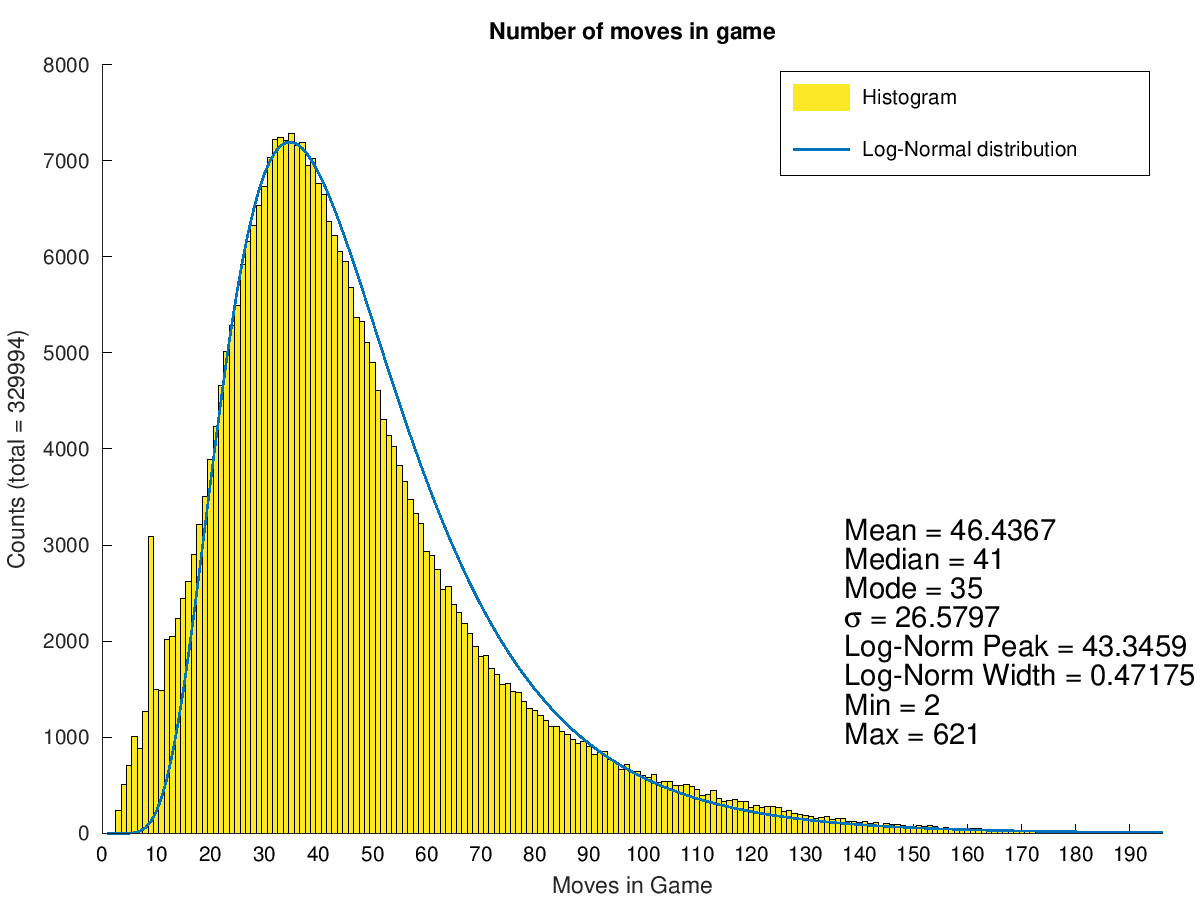
\includegraphics[width=0.7\textwidth]{game_length_log_norm_distribution.png}
	\caption{The distribution of the number of moves in a game with a log-normal fit. The Log-Norm parameters listed are \(M\) for the Peak parameter and \(S\) for the Width parameter. To obtain a better fit, only games longer than 15~moves were considered, as shorter games were primarily by ill-adapted AIs (especially the spike at 9-move games), especially at the beginning of the gene pool run.}\label{log-norm-plot}
\end{figure}

If the number of moves left in the game is greater than the number of moves that will result in a clock reset, then the latter will determine how much time will be used. In a game with, say, 40/5~time control, where five minutes are added to the clock every 40~moves, every 40th move can use all the remaining time since an extra five minutes will be added after the move. Whatever the final number of moves left is used, the time on the clock is divided by that number to determine how much time to take to choose a move.

When choosing a move from the current board, the amount of time to consider a move is equal to the amount of time left for this board position divided by the number of legal moves left to consider. This naturally limits the depth of search while allowing deeper searches for positions with fewer legal moves, which are often a series of forced moves due to check and so deserve deeper inspection. If a move examination is cut off early for whatever reason (e.g., a game-ending move is found or through alpha-beta pruning), then the remaining time is available for as yet unexamined moves.

An effective chess player needs to look at the consequences of a move to decide if a move is good. In order to decide how far to look ahead (and if there is time remaining to examine this move), at each step, the AI divides the number of legal moves in the board position after the move under consideration by the number of positions it can examine per second.
\[
T = k\frac{N_{\textrm{legal}}}{v}
\]
where \(T\) is the time needed to look ahead on this move, \(N_{\textrm{legal}}\) is the number of legal moves on the board after the move is made, \(v\) is the rate of position examinations, and \(k\) is a genetically determined speculation constant that adjusts the amount of time to use. The speed \(v\) is determined by counting the number of positions evaluated (leaf nodes in the game tree) and dividing by the amount of time spent evaluating during the previous move. If the time \(T\) is less than the time allocated for the move, the algorithm looks ahead (the search function recurses) to examine the moves the opponent can make in response. Otherwise, it evaluates the current position and moves on to the next legal move.

In order to force every move to be examined to a useful depth, a minimum depth is computed based upon an estimate of how many effective moves there are on a random board. By ``effective'' move, I mean one that unlikely to be pruned from the search tree. If the effective move estimate is less than the actual number of legal moves, then the search can go deeper than one would expect based on a more realistic estimate because it is expected that many move variations will be skipped due to pruning. The computation starts with the observation that, in a game tree of depth \(D\) and branching factor \(B\), the number of leaf nodes that will be evaluated is
\[
N = B^D.
\]
Since the number of leaf nodes greatly outnumbers the non-leaf nodes and the time to evaluate a node is much greater than the time to pass through a non-leaf node, only these nodes matter. Then, if nodes can be evaluated at a rate of \(v\) nodes per second and time \(T\) is allocated for choosing a move, then
\[
N = vT,
\]
which results in
\[
vT = B^D \implies D = \frac{\log{vT}}{\log{B}}.
\]
If, during a search, the AI has the option to search deeper into the game and the current depth is less than \(D\), then it will choose to go deeper.

\subsubsection{Opening Move Gene}
This gene keeps a list of opening for for both black and white: one move for white to play first, and one move for each of white's first moves. For example, if a genome file has the entry \code{Nc3: e5}, then if that player is playing black and the opponent makes the move Nc3, then the player will make the move e5 in response. If the entry had instead been \code{Nc3: -}, then the player would do a normal minimax search for a move. Mutation consists of replacing the right-hand side of a randome entry in the list with a random choice another move (including none).

\subsection{Board-Scoring Genes}\label{board-score-section}

These genes are used to give a score to a board state. The higher the score, the more desirable the moves that lead to this board. The score is calculated by
\[Score = \sum_g Priority(g) \times Score(g,B)\]
where \(g\) represents each gene, \(Priority(g)\) is a genetically determined scalar multiplicative factor that determines how much the gene's score of the board influences the final score, and \(Score(g,B)\) is the result of the scoring procedure of that gene on a given board \(B\).

Since it is not only important to find position that are advantageous to the player, but also disadvantageous to the opponent, the final heuristic score for a board position is given by
\[Heuristic\ Score = Score(Player) - Score(Opponent).\]

In general, the scoring function outputs of each gene are scaled so that a typical board state gets a score between zero and one. For example, the Freedom to Move Gene divides the number of legal moves by a large number that represents slightly more legal moves than would be found on most chess boards (128 was chosen to be large enough and for fast division). This way, the priorities of genes can be easily compared as evolution progresses.

\subsubsection{Total Force Gene}\label{total-force}
This gene sums the strength of all the player's pieces on the board according to the Piece Strength Gene (see Section~\ref{piece-strength}). The score returned is divided by the total value of the starting set of pieces (8~pawns, 2~rooks, 2~knights, 2~bishops, 1~queen, and 1~king) so that the result is between~0 and~1.

Since there is always a black king and a white king on the board, the king values cancel in this gene's scoring method. So, the king value is only determined by the Opponent Pieces Targeted Gene (Section~\ref{opponent-pieces-targeted}). This may be interpreted as the value of putting the other player in check.

\subsubsection{Freedom to Move Gene}
This gene counts the number of legal moves in a position and divides it by a large number (128, as noted in Section~\ref{board-score-section}) to bring the maximum score near one.

\subsubsection{Pawn Advancement Gene}
This gene measures the progress of all pawns towards the opposite side of the board.
\[S = \frac{1}{8}\sum_p \left|\frac{rank(p) - home(p)}{5}\right|\]
Here, \(S\) is the total score, the sum is over all pawns \(p\) of the scoring side, \(rank(p)\) is the rank position of the current pawn, and \(home(p)\) is the home rank of the pawn (2~for White and~7~for Black). The division by~5 (the farthest a pawn can advance before promotion) and the division by~8 (the maximum number of pawns) normalize the score to be between~0 and~1.

\subsubsection{Passed Pawn Gene}
The gene counts the number of pawns that cannot be stopped or captured by an opponent's pawns. That is, a pawn is a passed pawn if there are no pawns ahead of it in its file or any directly adjacent files. Partial points are awarded for pawns that have fewer pawns ahead than usual (\(1/3\) for each free column ahead of mid-board pawns, \(1/2\) for for pawns on the edge).

\subsubsection{Opponent Pieces Targeted Gene}\label{opponent-pieces-targeted}
This gene sums the total strength (as determined by the Piece Strength Gene) of the opponent's pieces currently under attack. The returned result is divided by the total score of pieces at the start of the game, similarly to the Total Force Gene.

Interestingly, since both kings are always on the board, they always cancel each others effect in the Total Force Gene, leaving this gene alone to drive their strength value. The result of this is discussed in the results section (Section~\ref{piece-strength-with-king}).

\subsubsection{Sphere of Influence Gene}
This gene counts the number of squares attacked by all pieces. Bonus points are awarded if the square can be attacked with a legal move. That is, if a piece cannot reach a square in one move (perhaps because such a move is blocked by another piece), then that square is still counted as falling under the influence of the side owning that piece. Further bonus points are awarded based on how close the attacked square is to the king.

The effective formula for the score of this gene can be expressed as
\[score = \sum_s legal(s)\left(1+\frac{KTF}{1+distance(s,king)}\right)\]
where the sum is over all squares \(s\) on the board. The function \(legal(s)\) returns~0 if \(s\) is not attacked at all, or one of two genetically determined factors depending on if the the attack is legal (ignoring checks or pins) or not. (These two factors are normalized so that the sum of their absolute values is one.) An illegal move is one that is blocked by another piece. The term \(KTF\) is the king target factor and is a genetically determined weight that adjusts the importance of attacking squares close to the opposing king. The function \(distance(s_1, s_2)\) gives the distance between two squares in king moves and is equal to the maximum of the difference in file or rank between the squares. In the formula above, \(king\) represents the square the opposing king occupies.

\subsubsection{King Confinement Gene}
This gene tracks the manner in which the king is prevented from moving. In scoring a board, this gene counts the squares the king can reach given unlimited consecutive moves that do not land on attacked squares or are occupied by pieces of either side. The count is divided by 64 to give a score between zero and one. The priority of this gene is usually slightly negative at the beginning of the game (to encourage hiding the king away) and higher at the end of the game (to encourage the king to escape from restricted areas).

\subsubsection{King Protection Gene}
This gene counts the squares that have access to the king by any valid piece movement and are unguarded by that king's other pieces. In other words, it measures how exposed the king is to hypothetical attacks. A higher score means a less exposed king.

\subsubsection{Castling Possible Gene}
This gene returns a positive score to indicate that castling is possible in the near future. A higher score indicates that castling is closer to being a legal move due a castling move happening in the current variation. The score can vary based on a genetically determined preference for kingside or queenside castling. The numerical values of these preferences are normalized so that the sum of their absolute values is one.

\subsubsection{Pawn Islands Gene}
A pawn island is a group of pawns on neighboring files that are isolated from other pawns by empty files, and thus cannot help to defend pawns on other islands. This gene calculates the average number of pawns per island with the assumption that a greater number of islands with fewer pawns each is unwanted.

\subsubsection{Stacked Pawns Gene}
This gene counts the pawns that have a pawn of the same color ahead of them in the same file. The motion of these pawns is limited by the pawn in front. The score returned is the negative of the count since stacked pawns are generally considered to be disadvantageous.

\subsubsection{Checkmate Material Gene}
This gene returns a score of one if the scoring side has enough pieces to checkmate a lone king. Otherwise, it returns zero. This should help avoid piece trade-offs resulting in one side having a material advantage but unable to checkmate---king and knight vs\@. king and pawn, for example.

\subsubsection{Pawn Structure Gene}
This gene scores how pawns are defended. For each pawn on the side being scored, it gives one score to pawns that are guarded by other pawns, another score to pawns that are guarded by other pieces, and zero otherwise. I would estimate that pawns guarded by pawns would be scored higher, so diagonal chains of pawns would be favored to other structures.


\subsection{Genome File Format}\label{genome-file-format}
An example genome file is shown below. Each genome starts with the \verb|ID:| line and ends with \verb|END|. Each gene starts with \verb|Name:| and ends with a blank line. Each component of a gene is a single line and specified by a name followed by a colon and the numerical value. Spacing within the line does not matter.
\verbatiminput{../genome_example.txt}

In genome files that are the output of gene pool runs (see Section~\ref{gene-pool-section}) there will also be lines in the following format:

\vspace{1ex}
\verb|Still Alive: 2 : 759 849 872 896 899 901 902 903 # ... etc.|
\vspace{1ex}

This line lists the ID numbers (after the second colon) of the AIs that are still alive within gene pool \#2 (the number after the first colon).

\section{The Gene Pool: On the Care and Feeding of Chess AIs}\label{gene-pool-section}
In each generation, the players in the gene pool are shuffled in order to form pairs for a single game of chess. After the game, the two players mate to produce one offspring by picking each gene randomly from either parent with equal probability (recombination~\cite{recombination-wiki}). The offspring is then subject to a bout of the mutation procedure wherein a number genes are individually mutated (that number being controlled by periodically varying mutation rate specified in the gene pool configuration file shown in Section~\ref{gene-pool-config}). Finally, the offspring replaces the loser in the gene pool. If the game ended in a draw, the player to be replaced by the offspring is picked by coin flip. In the literature, this setup is classified under Evolutionary Strategies~\cite{evolution-strategy-wiki}, more specifically \((N/2+N)\)-ES~\cite{evolution-strategy-glossary}, where \(N\) is the population size after the chess games (half the initial population), \(/2\) refers to two parents producing one offspring through recombination, \(+\) means that the offspring compete with the parents (elitism), and the final \(N\) refers to how many offspring are generated to keep a constant population of \(2N\), half of which are killed off every generation.

In this procedure, some the genes of losing players are passed on and are only slowly weeded out since a single game does not actually provide much information about the fitness of any gene with respect to game play. The removal of individuals destroys genetic information. By ``information,'' I mean filtered genomes. If a gene (including small variations, given the continuous nature of these genotypes) is present is a large percentage of the species, then that gene must have been present in a great number of AIs that were victorious in their games through many generations and many different opponents. Genes found in losing organisms slowly fade away as their host organisms fail to survive long enough reproduce multiple times. On average, a gene from a losing AI will be present in 0.5~AIs (50\% chance of being passed on) in the next generation; a gene from a winning AI will be present in 1.5~AIs (1.0 from the parent and another 0.5 from the 50\% chance of being passed on) in the next generation.

One final means of preventing gene pool stagnation and preserving genetic diversity is to limit the amount of shuffling when creating matchups. The order is randomized, but most AIs end up near where they started. This way, widely separated AIs can evolve in independent communities. An example is shown in Figure~\ref{gene-pool-divergence}.

\begin{figure}[htb]
	\centering
	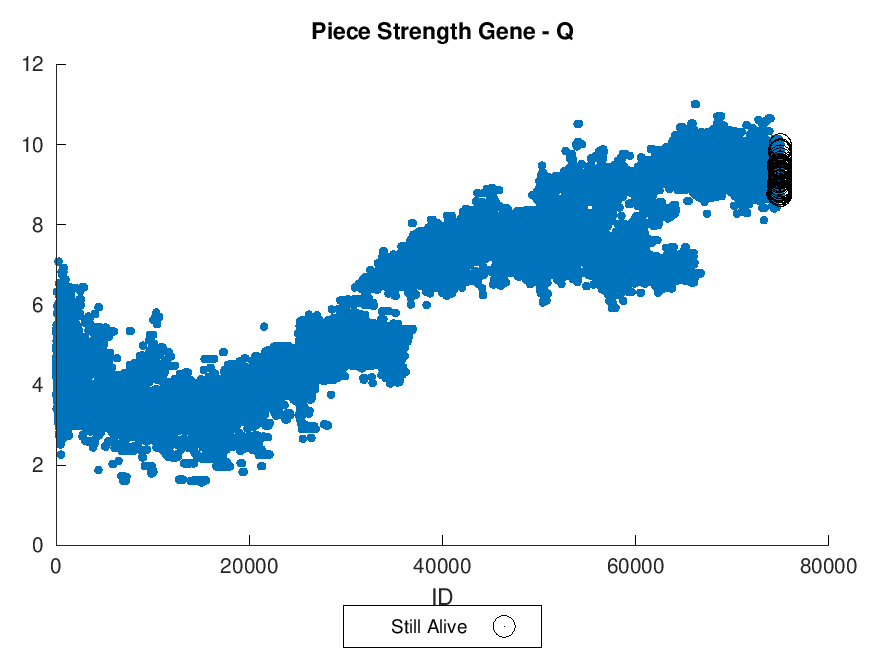
\includegraphics[width=\textwidth]{divergence-example}
	\caption{An example of diverging communities in a single gene pool (\(N=100\)). Near ID 35,000, a small offshoot community with a larger queen value can be seen to grow and eventually take over the whole pool. Near ID 60,000, the pool can be seen to split in half with the higher queen value again winning out.}\label{gene-pool-divergence}
\end{figure}

On Linux, the gene pool can be paused by pressing Ctrl-z. After the key press, the currently running games will finish and the results recorded before pausing. Pressing Ctrl-c exits the program immediately without waiting for current games to finish. To exit the program after the current round of games finish, pause first with Ctrl-z, then exit with Ctrl-c.

On Windows, pressing Ctrl-c exits the program after the current round of games is finished and recorded. Pressing Ctrl-c twice ends the program immediately without waiting for current games to finish.

\subsection{Gene Pool Configuration File}\label{gene-pool-config}
A gene pool is configured with a text file that is referenced in the program starting arguments (see Section~\ref{running}). An explanatory example gene pool configuration file is presented below.
\verbatiminput{../gene_pool_config_example.txt}

\subsection{Gene Pool Terminal Output}
An example of typical output during a gene pool run is shown below. First, some general information about the pool is shown, then the results of the random matchups, and finally the new makeup of this gene pool in the aftermath of the games. If \code{output volume} is set to \code{quiet}, then the game matchups and gene pool population and standings will not be printed to the screen.
\begin{verbatim}
Gene pool size: 100  Gene pool file name: pool.txt
Games: 6000  White wins: 3402  Black wins: 2511  Draws: 87
Rounds: 2170  Mutation rate phase: 70 (10/90)
Mutation rate: 2  Game time: 6.65 sec

106514 vs 106495: Black (Time forfeiture)
106531 vs 106513: White (White mates)
106511 vs 106479: Black (Black mates)
106392 vs 106457: None (Insufficient material) --> 106392 dies
106516 vs 106497: None (Threefold repetition) --> 106516 dies
106532 vs 106530: White (White mates)
106529 vs 106433: White (White mates)
106533 vs 106534: White (White mates)
... etc. ...

     ID   Wins  Draws
 106457      2      3
 106479      4      0
 106495      1      2
 106497      1      2
 106529      1      0
 106531      1      0
 106532      1      0
 106533      1      0
 106549      0      0
 106550      0      0
 106551      0      0
 106552      0      0
 106553      0      0
 106554      0      0
 106555      0      0
 106556      0      0
... etc. ...
\end{verbatim}


\section{Some Consistent Results (in rough order of discovery)}

Here are a few results that are reliably reproduced in multiple simulations. In these runs, there were three gene pools with 16~players each (so the number of games equaled the number of processors on my computer, i.e.,~8). Each game is played with 30~seconds per side for the entire game with no increment.

\subsection{Piece values are rated in near-standard order.}
In descending order of valuation by a Genetic\_AI\@: Queen, Rook, Bishop and Knight nearly equally, and Pawn. As time goes on,there is a lot of variation, especially in the relative order of the Rook, Knight, and Bishop. But, the standard order is preserved for the most part, as can be seen in Figure~\ref{piece-value-plot}.
\begin{figure}[htb]
	\centering
	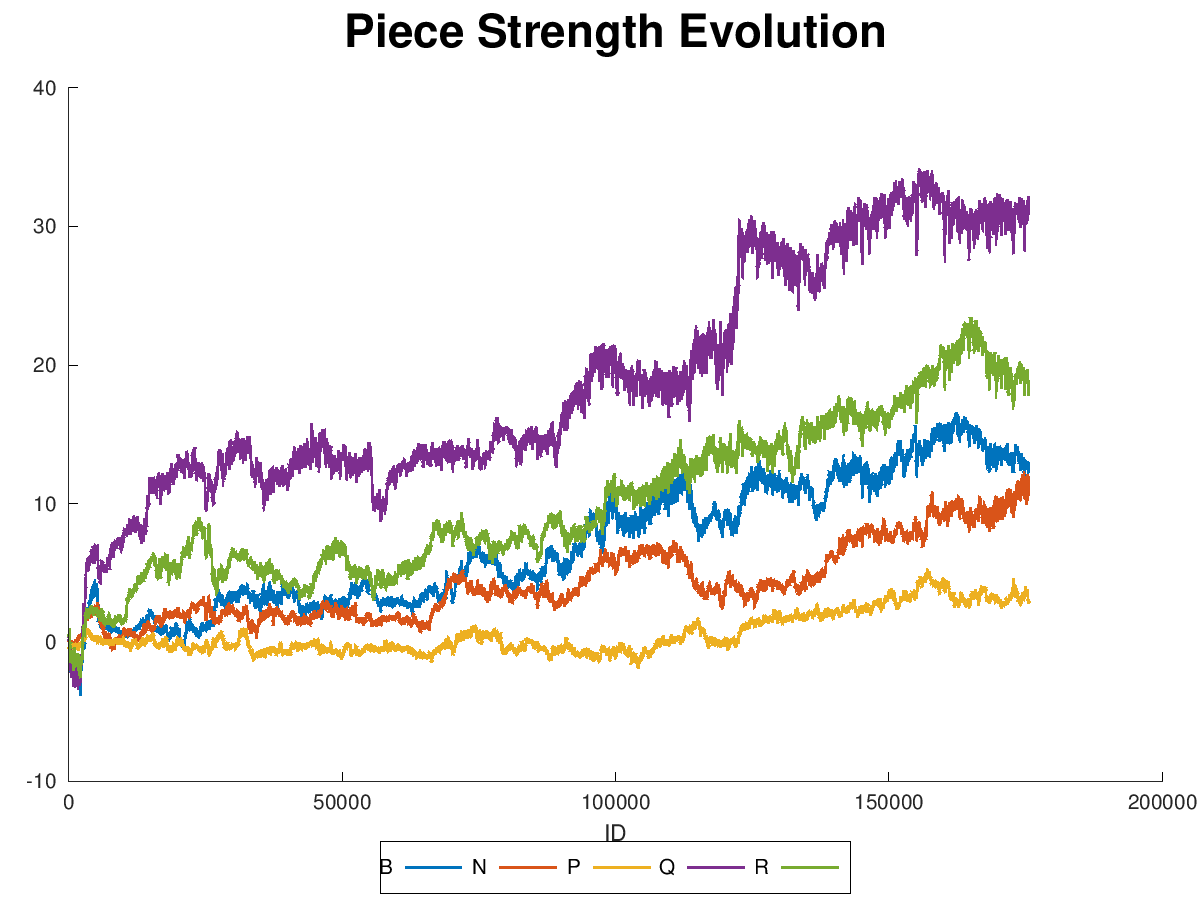
\includegraphics[width=\textwidth]{pawn-crash-strength-plot}
	\caption{The evolution of the value of pieces to the AIs.}\label{piece-value-plot}
\end{figure}

\subsubsection{Piece Strengths with the king}\label{piece-strength-with-king}

After assigning the king a strength entry in the Piece Strength Gene (see Section~\ref{piece-strength}), the other pieces retained their relative values, but the king evolved a very negative value. See Figure~\ref{piece-strength-with-king-plot}.
\begin{figure}[htb]
	\centering
	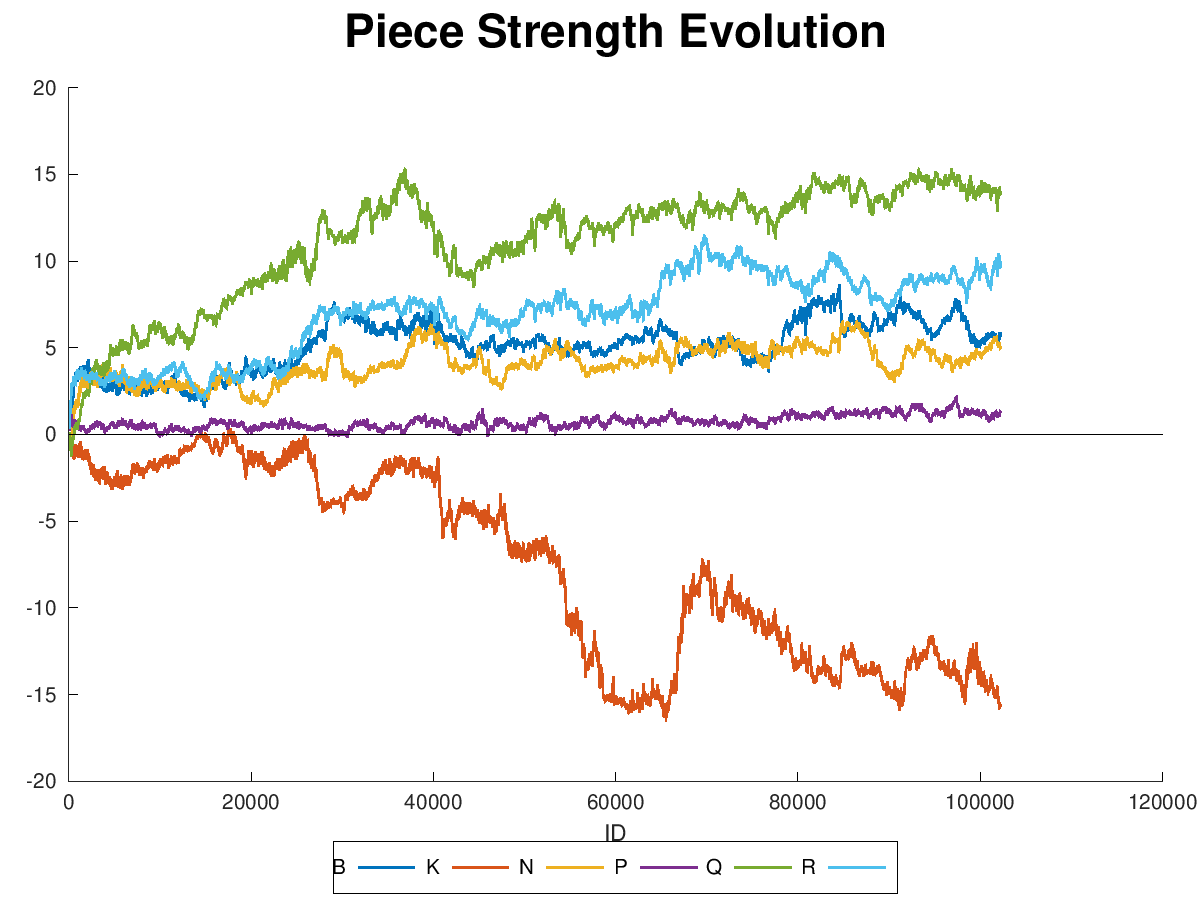
\includegraphics[width=\textwidth]{piece-strength-with-king-plot}
	\caption{The evolution of piece strengths after adding an entry for the king.}\label{piece-strength-with-king-plot}
\end{figure}

My current guess is that the king entry is affected by the Opponent Pieces Targeted  Gene and the Look-Ahead Gene---specifically the Capturing Speculation Constant. A large value for the Capturing Speculation Constant means that the board position that is actually evaluated has a smaller chance of having pieces threatened with capture. It is even less likely that the opponent's king is in check since this usually results in a reduced number of moves available, making recursion to the next move more likely. Thus, an evaluated board position with only the king in check is see as rather worthless unless offset by an attack on another piece that will probably result in capture. The king cannot be captured, so attacking it had better serve some other purpose. A similar evolution is seen in the Sphere of Influence Gene in that the King Target Factor is often negative.

This conclusion is corroborated by the King Target Bonus in the Opponent Pieces Targeted Gene (see Section~\ref{opponent-pieces-targeted}), which always has a negative or near-zero value that causes a preference for piece arrangements that attack more of the board away from the king.

\subsection{White has an advantage.}

Of the games ending in checkmate, white wins about 10\% more often than black. Figure~\ref{win-lose-plot} shows that the advantage is persistent through almost the whole of a long gene pool run. Wins by time are shared by black and white equally (see Figure~\ref{game-ending-plot}).
\begin{figure}[htb]
	\centering
	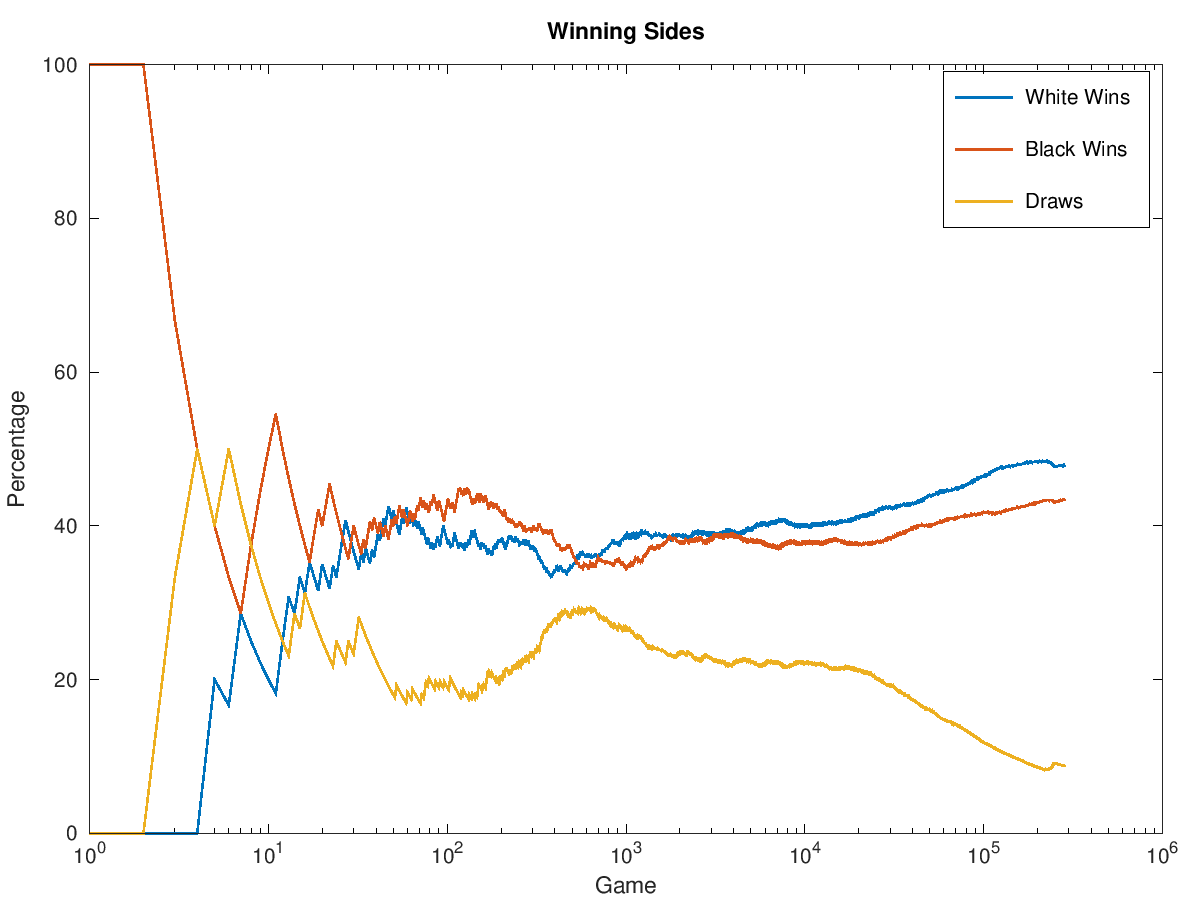
\includegraphics[width=\textwidth]{win-lose-plot}
	\caption{The percentage of games won by white, black, or neither over the course of a gene pool run. The advantage that white has over black seems persistent. Also, as the AIs evolve, the rate of draws decreases, presumably because they evolve a genome that can tell the difference between a good and bad position.}\label{win-lose-plot}
\end{figure}

\subsection{The Total Force Gene always dominates.}\label{total-force-result}

That the Total Force Gene dominates is fairly predictable. Highly skilled human players will usually resign after the loss of a minor (bishop or knight) piece without compensation.

\subsection{The Queen is the most popular piece for promotion.}

Even when the Piece Strength Gene has not been tuned at all, the queen is the overwhelming favorite, followed by the rook, then bishop, and finally the knight. In human games, only the queen and knight are chosen since they have different move patterns. If you need at least a rook or bishop, you might as well take a queen since that piece provides both. Only the knight provides a viable alternative (usually to avoid a stalemate if the queen was chosen).

As an example, the following is a count of all promotions in a gene pool run after more than 300,000 games.
\begin{center}
\begin{tabular}{l r}
	Piece & Promotions \\
\toprule
	Bishop & 2232  \\
	Knight  &  1648 \\
	Rook    &  7215 \\
	Queen  & 146664 \\
\end{tabular}
\end{center}


\subsection{Threefold repetition is the most common draw.}

Most games with human players end in a draw when neither side can force an advantage. This happens when one side can block a crucial move (e.g., a pawn promotion) and the other side cannot remove this block. Since the blocking player does not have a reason to move, he can just repeat moves to maintain the block. This would lead to threefold repetition if most players did not verbally draw the game beforehand. Since these Genetic AI players don't offer or accept draws, they play out all the repetitions, resulting in what is seen in Figure~\ref{game-ending-plot}.

\subsection{The Look Ahead Gene is a late bloomer.}

The plot in Figure~\ref{game-ending-plot} shows the counts of how games end.
\begin{figure}[htb]
	\centering
	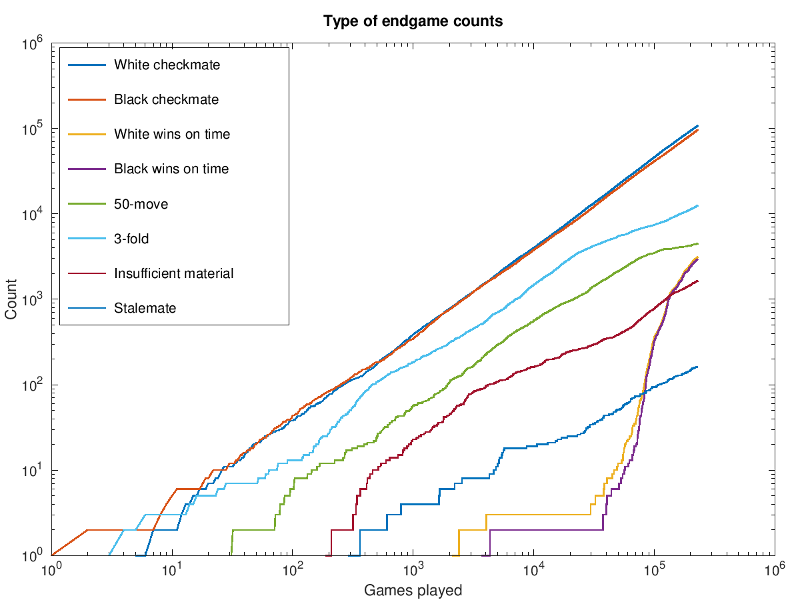
\includegraphics[width=\textwidth]{game-endings-log-plot}
	\caption{A log-log scale of the percentage of games with various endings. Note that the time forfeits don't get going until about 30,000 games in.}\label{game-ending-plot}
\end{figure}
It seems that the Look Ahead Gene does not experience significant evolutionary pressure until the board-scoring genes have been tuned to a semi-decent state. My hypothesis is that if the board-scoring function is not able to tell a good position from bad, then looking ahead only increases the risk of losing by time forfeiture with no benefit. However, when the board-scoring genes are in a decent state, the increase in look ahead is very quick. This leads to a rapid increase in the rate of deaths by running out of time, but apparently this is worth the risk as those who are more conservative with their time lose to those who see farther ahead.

\subsection{The Sphere of Influence Gene typically counts legal moves as having lower value than other moves.}

This was unexpected. I thought that the legal moves would count more since they present a greater threat to the opponent. You cannot capture your opponent's Queen if your own King is in check. Perhaps Genetic\_AIs find this gene more useful as a forward-looking view of the game. Or, the Opponent Pieces Targeted Gene relieves this gene of having to consider legal moves.



\begin{thebibliography}{99}

\bibitem{pgn-file-format}
\url{http://www.thechessdrum.net/PGN_Reference.txt}

\bibitem{fen-notation}
\url{http://www.thechessdrum.net/PGN_Reference.txt} Section~16.1

\bibitem{evolved-antenna}
G.S. Hornby, A. Globus, D.S. Linden, J.D. Lohn, ``Automated Antenna Design with Evolutionary Algorithms.'' AIAA

\bibitem{evolved-stellarator}
W.H. Miner, Jr., P.M. Valanju, S.P. Hirshman, A. Brooks, N. Pomphrey, ``Use of a genetic algorithm for compact stellarator coil design.'' IAEA Nuclear Fusion, Vol. 41, No. 9. 1185--1195

\bibitem{quiescence-ref}
\url{https://www.chessprogramming.org/Quiescence_Search}

\bibitem{laplace}
\url{https://en.wikipedia.org/wiki/Laplace_distribution}

\bibitem{iterative-deepening}
\url{https://www.chessprogramming.org/Iterative_Deepening}

\bibitem{log-norm-wiki}
\url{https://en.wikipedia.org/wiki/Log-normal\_distribution}

\bibitem{log-norm-chess-se}
\url{https://chess.stackexchange.com/a/4899/5819}

\bibitem{recombination-wiki}
\url{https://en.wikipedia.org/wiki/Genetic_recombination}

\bibitem{evolution-strategy-wiki}
\url{https://en.wikipedia.org/wiki/Evolution_strategy}

\bibitem{evolution-strategy-glossary}
\url{http://ls11-www.cs.tu-dortmund.de/~beyer/EA-glossary/node41.html}

\end{thebibliography}

\end{document}
